% \section{Introduction}
%
% - \texit{Ab initio} structure prediction is a balancing act between time spent to generate decoys and the quality of the final decoy set
% - \texit{Ab initio} structure prediction can only predict accurate structures with a subselection of fragments collective capturing the overall target fold
%
% - AMPLE requires decoys with the overall accurate fold yet enough diversity in the set to truncate to the conserved core
% - AMPLE typically succeeds with small to medium size fragments relative to the target sequence (20-50\%)
%
% This bares the question whether fragments extracted for \textit{ab initio} structure prediction are sufficient as \gls{mr} search models. This stems primarily on the assumption that fragment picking algorithms can identify fragments based on sequence features that are structurally similar to a sequence position in our target.
%
% - Something about the addition of contacts as unique feature for further identifying correct fragments
% - Something about differences to other fragment-\gls{mr} approaches

\section{Methods}
\subsection{Target selection}
Targets were manually chosen using favourable cases for this proof-of-principle study, i.e. resolution was chosen to be ~1.5\AA, target chain lengths were $<150$ residues, and only a single molecule is present in the asymmetric unit (\cref{table:ample_flib_target_properties}).

\begin{table}[H]
  \centering
  \caption{Overview of Flib target properties.}
  \label{table:ample_flib_target_properties}
  \begin{tabularx}{\textwidth}{X X X X X X}
      \hline
      \textbf{Target} & \textbf{Fold} & \textbf{Chain Length} & \textbf{Resolution (\AA)} & \textbf{Nmol/ASU} &
\textbf{Space Group} \\ 
      \hline
      1aba & mixed \textalpha-\textbeta & 87    & 1.45 & 1      & P $2_1$ $2_1$ $2_1$   \\
      1lo7 & mixed \textalpha-\textbeta & 141   & 1.50 & 1      & I $2$ $2$ $2$         \\
      1u06 & all-\textbeta              & 62    & 1.49 & 1      & P $2_1$ $2_1$ $2_1$   \\
      5nfc & all-\textbeta              & 147   & 1.59 & 1      & P $2_1$ $2_1$ $2_1$   \\
      \hline
  \end{tabularx}
\end{table}

\subsection{Fragment picking using Flib}
Fragments for this study were picked using the Flib algorithm \cite{De_Oliveira2015-ba}. 

Flib requires four inputs: the predicted secondary structure, predicted torsion angles, predicted residue-residue contact prediction and a copy of the \gls{pdb}. The secondary structure for each target was predicted using PSIPRED v4.0 \cite{Jones1999-fi} with default parameters. The torsion angles were predicted using SPIDER2 \cite{Heffernan2015-wp} with default parameters, and residue-residue contact pairs using METAPSICOV v1.04 \cite{Jones2015-wp} with default parameters. HHBLITS v2.0.16 \cite{Remmert2011-ze} with database version \texttt{uniprot20\_2016\_02} was used by METAPSICOV to generate the \gls{msa} for contact prediction of each target sequence. BLASTp v2.2.31+ \cite{Altschul1990-nc,Camacho2009-ue} was used by PSIPRED with the UNIPROT database version \texttt{uniref90-2016\_06}. The local copy of the \gls{pdb} for fragment picking was downloaded on August 11, 2016.

Two modifications were made to the default Flib v1.01 (\url{https://github.com/sauloho/Flib-Coevo}) protocol. The first focuses on exclusion of fragments with $>90$\% helical content (assigned by DSSP \cite{Frishman1995-ns}). The second modification was to allow fragments with \gls{rmsd} $>10.0$\AA\ to be considered.

Two-hundred fragments were picked per target sequence position. Top-$L$ or $L/2$ contact pairs were considered from both METAPSICOV STAGE 1 and STAGE 2 predictions with a minimum sequence separation of either 6 or 12 residues. Helical fragments were either in- or excluded and only fragments with length between 6 or 12 residues up-to 63 residues considered. Overall, this generated 16 fragment libraries per target.

Each fragment library was then filtered to remove homologs. Hereby, BLASTp and HHpred \cite{Soding2005-sx} searches were conducted to identify homologous PDB entries. The BLASTp search was performed identically to \cite{De_Oliveira2015-ba}. The HHpred search parameters were identical to the MPI-Toolkit \cite{Biegert2006-ny} webserver version (\url{https://toolkit.tuebingen.mpg.de/}). Fragments derived from PDB entries identified by BLASTp and HHpred (probability score of $\geq20.0$) were excluded from the fragment libraries.

All fragments per target were then grouped by their length. Subsequently, they were ranked twice by Flib scores and \gls{rmsd} values, and the best fragment selected. Fragments of the same template structure consisting of the same region with varying flanking residues were kept, if they were ranked top for each fragment length group. Finally, the coordinates for the selected fragments were extracted and two files created for each, one containing the backbone atoms and the other containing all atoms.

\subsection{\acrlong{mr} in MrBUMP}
The previously extracted fragments were subjected to the \gls{mr} pipeline MrBUMP \cite{Keegan2008-hk}. The latter uses PHASER \cite{McCoy2007-bf} for \gls{mr}, REFMAC5 \cite{Murshudov2011-we} for refinement and SHELXE \cite{Thorn2013-ir} for density modification and main-chain tracing. MrBUMP default parameters were used with exception of the PHASER RMS estimate. \gls{mr} was attempted for each coordinate file with a PHASER RMS value of 0.1, 0.6, and 1.0.

The \gls{mr} success for each search model was assessed by SHELXE scores only, whereby a \gls{cc} score of $\geq25.0$ combined with an \gls{acl} score of $\geq10.0$ is required.


\section{Results}
\subsection{Precision of Flib dependency data}
The first part of this study is to analyse the data dependencies required by the Flib fragment picking algorithm. This analysis is important given that the Flib fragment picking heavily relies on the individual features in the selection and scoring of each individual fragment \cite{De_Oliveira2015-ba}. Poor data at this stage could lead to poor fragments unsuitable for \gls{mr} trials given that high accuracy, i.e. an low \gls{rmsd} value between the search model and target, is required.

The secondary structure prediction highlighted high precision between each target's prediction and the DSSP-assigned \cite{Frishman1995-ns} secondary structure of the target reference structure (\cref{fig:ample_flib_psipred}). The three targets with \gls{pdb} identifiers 1aba, 1lo7 and 1u06 have secondary structure predictions with a precision of $>72$\%. The fourth target, 5nfc, shows comparatively poor precision of 52.4\%. However, almost all secondary structure features are correctly identified.

\begin{figure}[H]
	\centering
	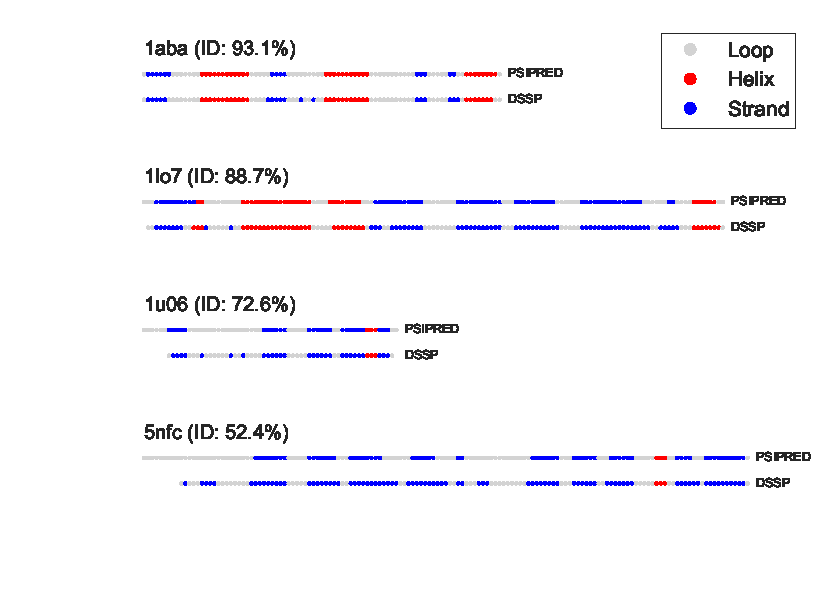
\includegraphics[width=\textwidth]{ample_flib_psipred.pdf}
	\caption[PSIPRED schema for Flib targets]{Schematic comparison of PSIPRED \cite{Jones1999-fi} secondary structure prediction and DSSP \cite{Frishman1995-ns} assignment. Percentage identity is provided next to each identifier.}
	\label{fig:ample_flib_psipred}
\end{figure}

The contact prediction data for METAPSICOV STAGE 1 and STAGE 2 predictions demonstrate the high precision scores achievable by this algorithm (\cref{table:ample_flib_contact_precision}). In this study, the top contact pairs at cutoffs \textit{L} and \textit{L/2} were provided to the Flib algorithm. All targets have precision scores for both sets of predictions at both cutoff levels of $>0.6$ (\cref{table:ample_flib_contact_precision}).

\begin{table}[H]
  \centering
  \caption[Contact prediction summary for Flib targets]{Precision scores for METAPSICOV \cite{Jones2015-wp} STAGE 1 and STAGE 2 contact predictions. Jaccard index calculated for the same contact pairs between METAPSICOV STAGE 1 and STAGE 2 predictions.}
  \label{table:ample_flib_contact_precision}
  \begin{tabularx}{\textwidth}{X X X X X X X}
      \hline
	  \multirow{2}{*}{\textbf{Target}} & \multicolumn{3}{c}{\textbf{\textit{L/2} contact pairs}} & \multicolumn{3}{c}{\textbf{\textit{L} contact pairs}} 	\\ \cline{2-7}
	  							&  	STAGE 1	& 	STAGE 2	& 	Jaccard 	& 	STAGE 1 	& 	STAGE 2 	& 	Jaccard	 	\\
	  \hline
	  1aba						&	0.884	&	0.884	&	0.303	&	0.713	&	0.759	&	0.513		\\
	  1lo7						&	0.857	&	0.957	&	0.308	&	0.738	&	0.837	&	0.446		\\
	  1u06						&	0.839	&	0.806	&	0.378	&	0.710	&	0.787	&	0.459		\\
	  5nfc						&	0.822	&	0.836	&	0.327	&	0.619	&	0.762	&	0.434		\\ 
	  \hline
  \end{tabularx}
\end{table}

Given the two prediction files, both show localised clusters of contact pairs suggesting
 secondary structure features found in the native protein structures (\cref{fig:ample_flib_cmaps}). However, METAPSICOV STAGE 1 predictions show a much higher frequency of singleton contact pairs, i.e. ones without a neighbouring contact pair.

\begin{figure}[H]
	\centering
	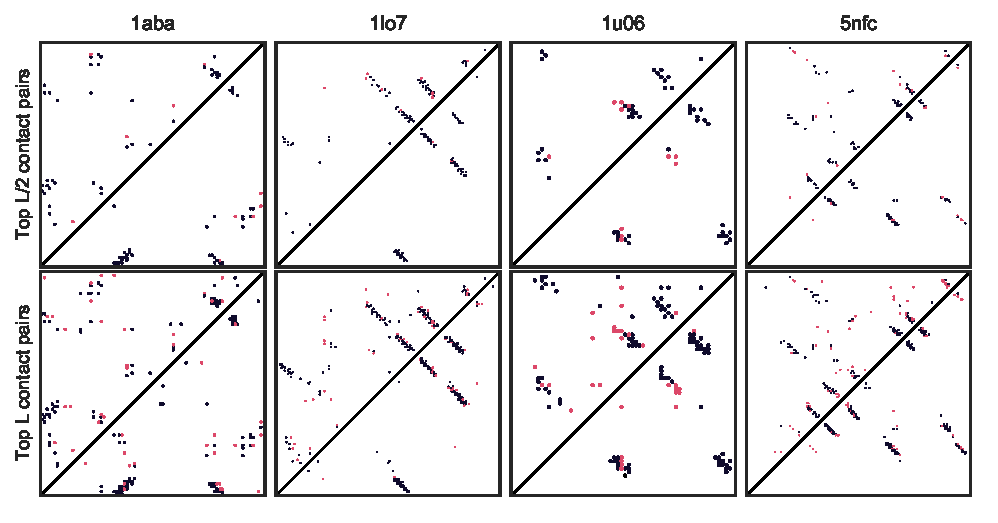
\includegraphics[width=\textwidth]{ample_flib_cmaps.pdf}
	\caption[Contact map comparison for Flib targets]{Comparison of $L/2$ and $L$ correctly (gray) and incorrectly (pink) predicted contact pairs for four Flib targets. Contacts were predicted using METAPSICOV STAGE 1 (top left) and STAGE 2 (bottom right) \cite{Jones2015-wp}. True and false positive contact pairs were identified using a 8\AA cutoff between C\textalpha\ (C\textbeta\ in case of GLY) atoms of a reference crystal structure.}
	\label{fig:ample_flib_cmaps}
\end{figure}

An analysis of the absolute difference of torsion angles between the SPIDER2 \cite{Heffernan2015-wp} prediction and a corresponding reference crystal structure highlight accurate predictions for three of four targets (\cref{fig:ample_flib_spider2}). The largest \gls{mae} of \textphi-angles across the four target sequences is $24.347^{\circ}$, and the largest \gls{mae} of \textpsi-angles is $45.459^{\circ}$ (\gls{mae} values for \gls{pdb} entry 1u06). The smallest \textphi-\gls{mae} is $13.822^{\circ}$ (\gls{pdb}: 1aba) and smallest \textpsi-\gls{mae} is $17.273^{\circ}$ (\gls{pdb}: 1lo7). Segments in sequence space with regular secondary structure, as predicted by PSIPRED \cite{Jones1999-fi}, result primarily in low \gls{mae} of torsion angles. In contrast, unstructured regions highlight much larger \gls{mae} values indicating the difficulty of predicted these regions. Noticeably, the \textpsi-\gls{mae} appears to be much larger in those regions than the \textphi-\gls{mae} for the same residue.

\begin{figure}[H]
	\centering
	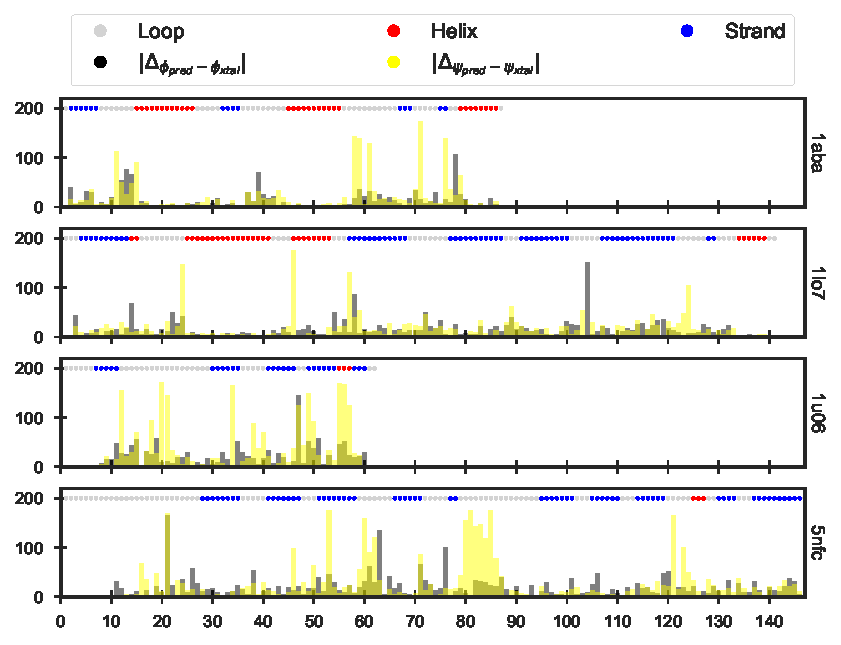
\includegraphics[width=\textwidth]{ample_flib_spider2.pdf}
	\caption[SPIDER2 torsion angle prediction analysis of Flib targets]{Comparison of \gls{mae} of torsion angles predicted by SPIDER2 and extracted from a corresponding \gls{pdb} structure. PSIPRED \cite{Jones1999-fi} secondary structure prediction provided alongside the \gls{mae} values.}
	\label{fig:ample_flib_spider2}
\end{figure}

\subsection{Flib fragment picking}

Sixteen Flib fragment libraries were picked for each protein target in this study. Each fragment library consisted of one permutation given altering input paramaters and contact prediction files.

Across all four targets, the Flib algorithm selected a total of 8,548,775 fragments (\cref{table:ample_flib_frag_summary}). The fragment libraries show similar statistics across the four protein targets despite the diversity in fold and chain lengths. The Flib score average falls at ~3,200 Flib score units with an average 9.0\AA\ \gls{rmsd}. Fragments for the alpha-spectrin SH3 domain (\gls{pdb} ID: 1u06) scored the lowest mean Flib score with 3035.50 units; however, the same target scored the worst by mean \gls{rmsd} with an average of 9.48\AA. In contrast, fragments picked for the sequence of the bacteriophage T4 glutaredoxin (\gls{pdb} ID: 1aba) achieved the best mean \gls{rmsd} of 7.85\AA\ given the second highest mean Flib score of 3217.49 units (\cref{table:ample_flib_frag_summary}).

\begin{table}[H]
  \centering
  \scriptsize
  \caption[Flib fragment characterics across four protein targets]{Summary of fragment statistics for Flib libraries selected for four protein targets. Count\textsubscript{H} corresponds to the count of fragments extracted from homologs.}
  \label{table:ample_flib_frag_summary}
  \begin{tabularx}{\textwidth}{X X X X X X X X X}
      \hline
      \multirow{2}{*}{\textbf{Target}} & \multirow{2}{*}{\textbf{Count}} & \multirow{2}{*}{\textbf{Count\textsubscript{H}}} & \multicolumn{3}{c}{\textbf{Flib score}} & \multicolumn{3}{c}{\textbf{\gls{rmsd}}} \\ \cline{4-9}
      		&			&			& Median 	& Mean 		& Sigma 	& Median 	& Mean 	& Sigma \\
      
      \hline
	  1aba	& 2,094,332	& 45,193	& 3061.05	& 3217.49	& 1405.71	& 7.70		& 7.85	& 3.81	\\
  	  1lo7  & 2,501,675	& 23,416	& 3187.44	& 3372.06	& 1497.49	& 9.00		& 9.43	& 4.61  \\
      1u06  & 1,136,435	& 60,456	& 2902.68	& 3035.50	& 1306.17	& 9.51		& 9.48	& 3.94	\\
      5nfc  & 2,816,333	& 48,839	& 2982.69	& 3127.00	& 1316.56	& 8.89		& 9.16	& 4.18	\\ 
      \hline
      Total	& 8,548,775	& 177,904	& 3049.31	& 3208.72	& 1397.20	& 8.68		& 8.96	& 4.25	\\ 
      \hline
  \end{tabularx}
\end{table}

A split of the per-target fragment libraries into their distinct conditions highlights the improved library quality of certain conditions with regards to the mean Flib score and \gls{rmsd} (\cref{fig:ample_flib_flibcond}). In particular, top-$L$ (6 residues sequence separation) METAPSICOV STAGE 1 contact predictions yielded the lowest for both metrics across all targets, which suggests this condition to be the most favourable for picking fragments. A comparison of the sequence separation, i.e. using all contact pairs or medium- and long-range ones only, strongly suggests much lower and thus more favourable scores for using all contact pairs. A very similar difference is noticeable for METAPSICOV STAGE 2 contact predictions (\cref{fig:ample_flib_flibcond}). Independent of the starting contact prediction, the most favourable condition for selecting fragments using Flib uses top-$L$ contact pairs with 6 residues sequence separation. The exclusion of idealised \textalpha-helical fragments did not affect the overall Flib score and \gls{rmsd} greatly ($max \Delta_{Flib}=25.87; max \Delta_{RMSD}=0.06$).

\begin{figure}[H]
	\centering
	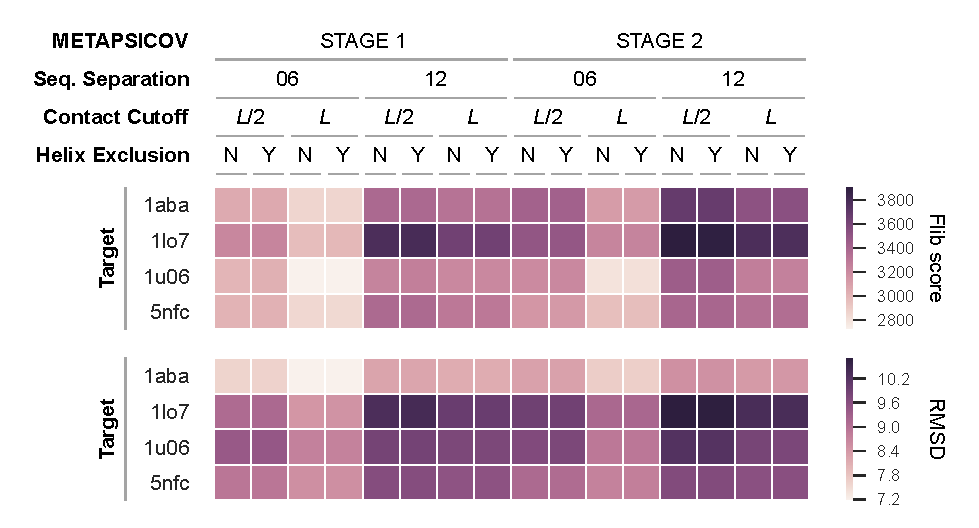
\includegraphics[width=\textwidth]{ample_flib_flibcond.pdf}
	\caption[Flib fragment library comparison]{Flib fragment library comparison for four targets highlighting the differences in mean Flib score and \gls{rmsd} by starting with different subsets of contact predictions. $L$ refers to the number of residues per target sequence. $Y$ refers to idealised \textalpha-helical fragment exclusion during fragment picking; $N$ refers to treating those fragments like all others.}
	\label{fig:ample_flib_flibcond}
\end{figure}

\subsection{Flib fragment selection for \acrlong{mr}}

One of the most important aspects of bypassing \textit{ab initio} structure prediction and using the relevant fragments directly as \gls{mr} search models is the selection of the fragments with the highest similarity between fragment and target structure. The Flib score - a cumulative metric judging the quality of a fragment - is the most obvious feature; however, it is unknown to-date whether a correlation between the Flib score and the fragment \gls{rmsd} exists. Taking all non-homologous fragments in this study, a first attempt was made to identify a correlation between a fragment's Flib score and \gls{rmsd}. The results presented here indicate towards a positive correlation between the Flib score and the corresponding fragment \gls{rmsd} for almost all fragments across the different target fragment libraries (\cref{fig:ample_flib_flibrelat}). However, a small fraction of fragments appear as outliers, not fitting the correlation of lower Flib scores corresponding to lower \gls{rmsd} values. On average, \textcolor{red}{XY}\% of fragments per library are contained in this outlier set.

\begin{figure}[H]
	\centering
	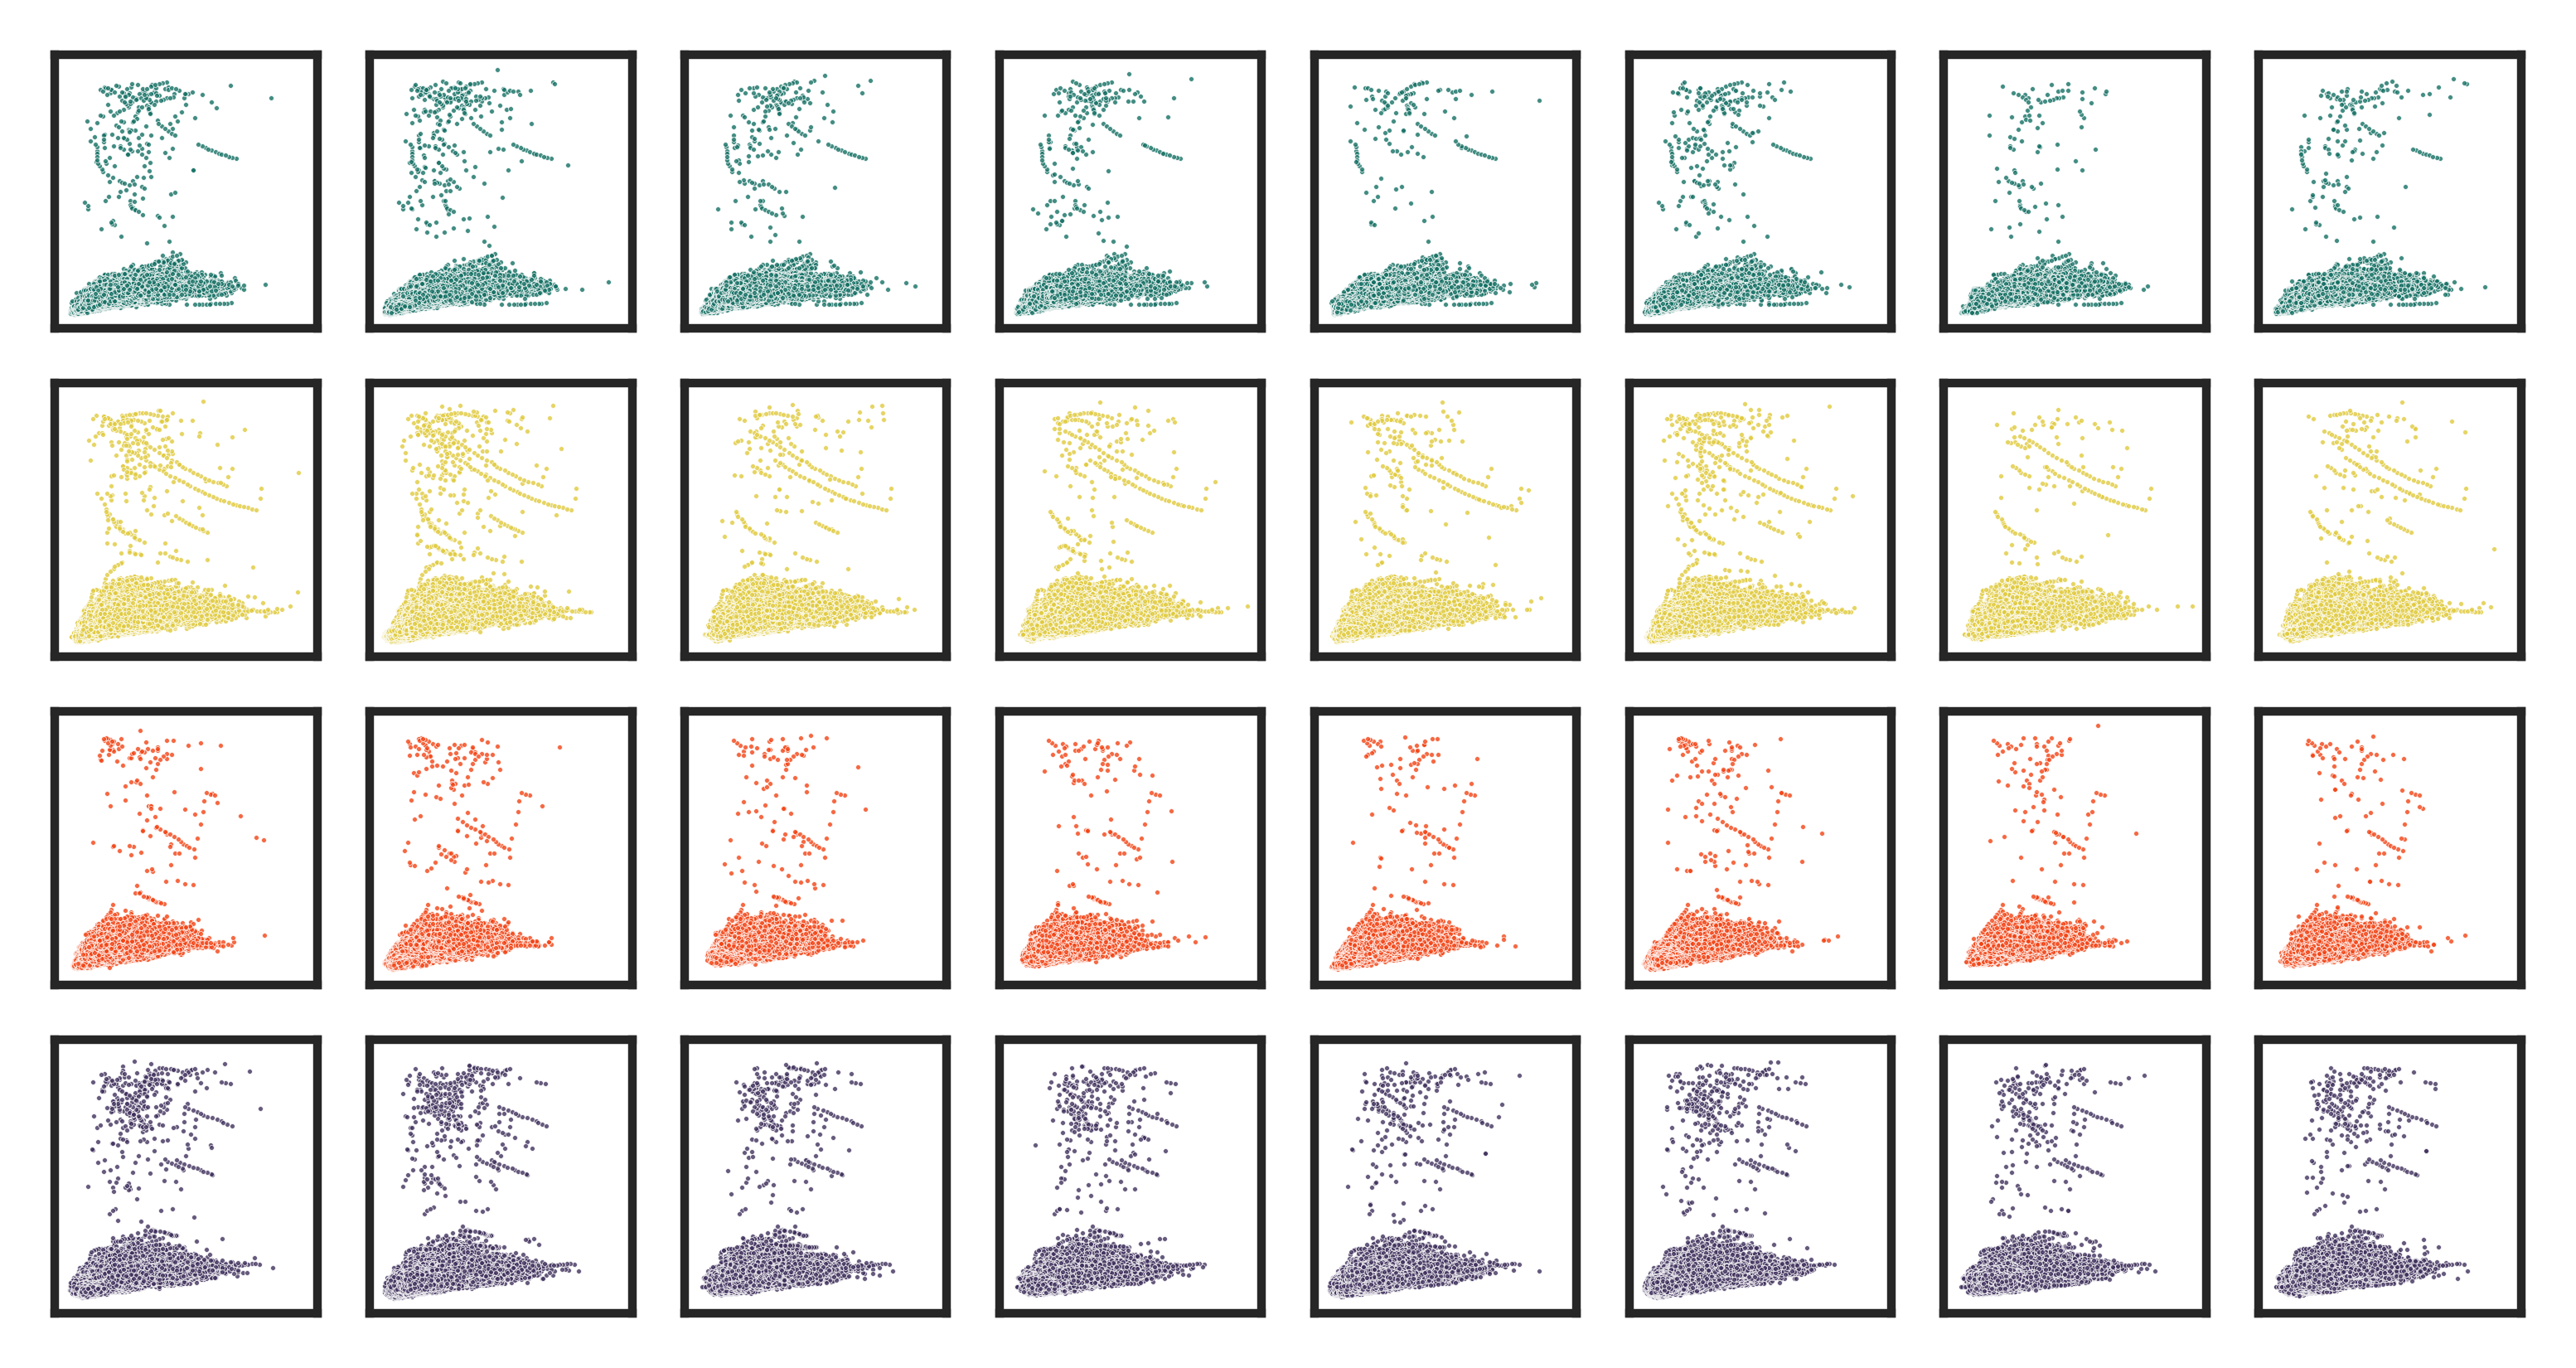
\includegraphics[width=\textwidth]{ample_flib_flibrelat.png}
	\caption[Correlation analysis for Flib score and \gls{rmsd}]{Scatterplot highlighting the positive correlation between fragment Flib scores (x-axis) and \gls{rmsd} values *. Four targets are illustrated: 1aba (green), 1lo7 (yellow), 1u06 (orange), and 5nfc (purple). Each column represents a different fragment picking strategy, and no fragment illustrated correpsonds to an idealised \textalpha-helix.}
	\label{fig:ample_flib_flibrelat}
\end{figure}

An analysis of the outliers for characteristics that would allow for their exclusion showed the randomness of their occurrence. These fragments contain all secondary structure types, span the entire target sequence and consist of a great range of peptide lengths. Furthermore, they occur in all fragment libraries, irrelevant of their original picking strategy. The only characteristic, which would be impossible to use \textit{a priori} is the fragments' \gls{rmsd} values, which are $>30$\AA. However, it is worth noting that the minimum Flib score in the outlier fragment set and the remaining fragment sets are distinctly different. The outliers' minimum extracted from all fragment sets is 993.02 Flib score units. In comparison, fragments with \gls{rmsd} $\leq30$\AA\ have a minimum \gls{rmsd} of 72.16, which suggests that the outlier fragments might not make it in the final selection.



